% !TEX encoding = UTF-8
% !TEX TS-program = pdflatex
% !TEX root = ../tesi.tex

%**************************************************************
\chapter{Metodi di risoluzione}
\label{cap:algoritmi}
%**************************************************************

\section{DFS}
\subsection{Descrizione}
Il primo algoritmo utilizzato per risolvere il nostro problema è stato il Depth First Search. È una strategia di ricerca non informata in quanto non si utilizzano informazioni aggiuntive sugli stati oltre alla definizione iniziale del problema.
Quindi l'algoritmo è solamente in grado di generare successori e distinguere se sono uno stato obiettivo o meno. \\
Questa strategia esplora tutti gli stati dell'albero di ricerca in profondità, cioè espande prima lo stato più profondo non ancora esplorato, ritornando indietro nel caso il cammino non porti a nessuno stato obiettivo in un numero finito di azioni. \\
Questo tipo di ricerca termina non appena trova il primo stato obiettivo, generando però, nel caso pessimo, una complessità temporale (numero di stati generati) di $\mathcal{O}(b^m)$ dove m è la massima lunghezza di un percorso e b il massimo numero di successori di uno stato, rendendo questo algoritmo poco efficiente.
\begin{figure}[h]
	\centering
	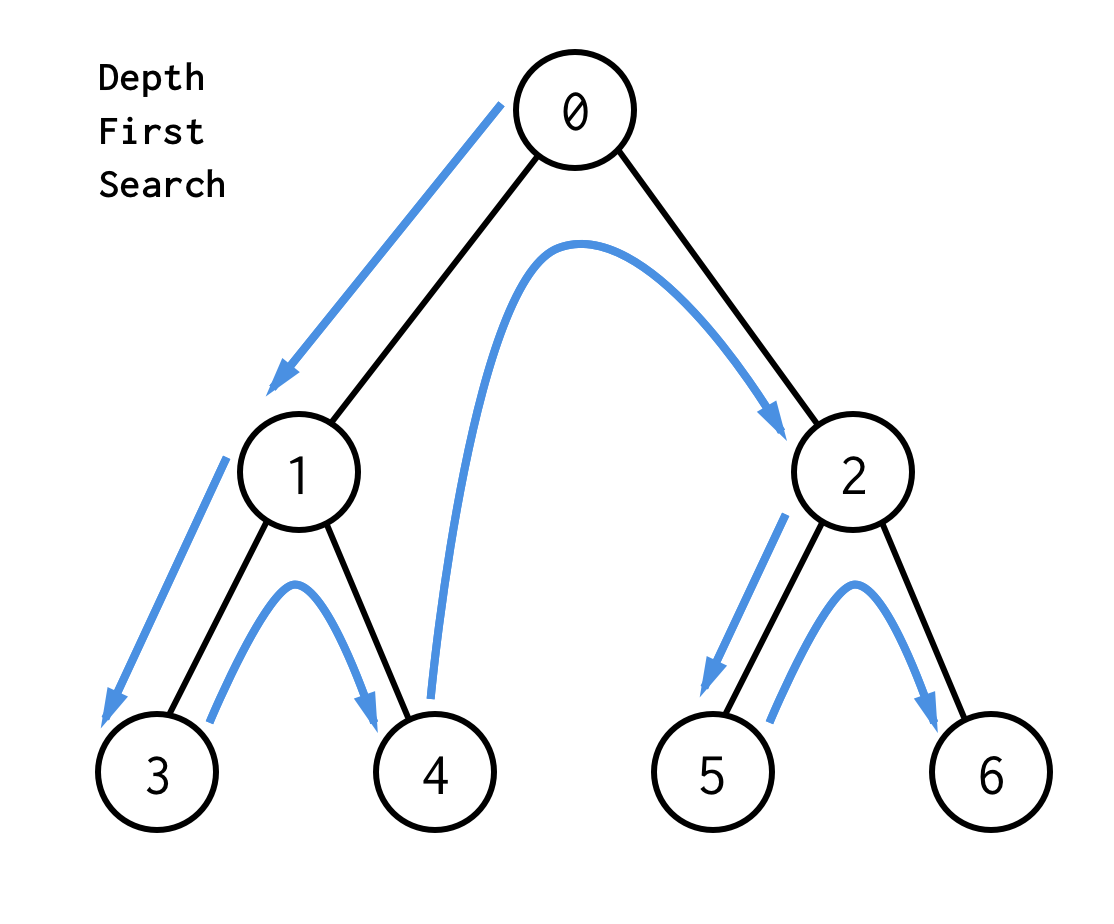
\includegraphics[scale=0.25]{immagini/dfs}
	\caption{Esempio di ricerca DFS}
	\label{fig:dfs}
\end{figure}

\subsection{Utilizzo}
Nel nostro caso l'algoritmo DFS è stato implementato in maniera ricorsiva, dove ogni stato rappresenta la configurazione attuale della griglia, intesa come forme già inserite e la loro posizione (coordinate all'interno della griglia). La configurazione iniziale della griglia rappresenta lo stato iniziale dal quale iniziale la ricerca in profondità.\\
I successori di ogni stato sono tutti i possibili posizionamenti, consistenti con l'assegnamento corrente (forme inserite e relativa posizione nella griglia), delle forme non ancora presenti nella griglia di gioco. Quindi l'algoritmo ad ogni passo sceglie la prossima forma da inserire, assegnandole il primo valore consistente nel suo dominio.
Qualora non ce ne fossero si ritorna allo stato precedente, espandendo un altro successore, fino ad arrivare ad uno stato obiettivo dove tutte le forme sono piazzate all'interno della griglia, in modo da riempirla totalmente.  \\
Essendo il nostro spazio di ricerca finito, l'algoritmo DFS ci assicura di ritornare sempre una soluzione al problema.
\begin{figure}[h]
	\centering
	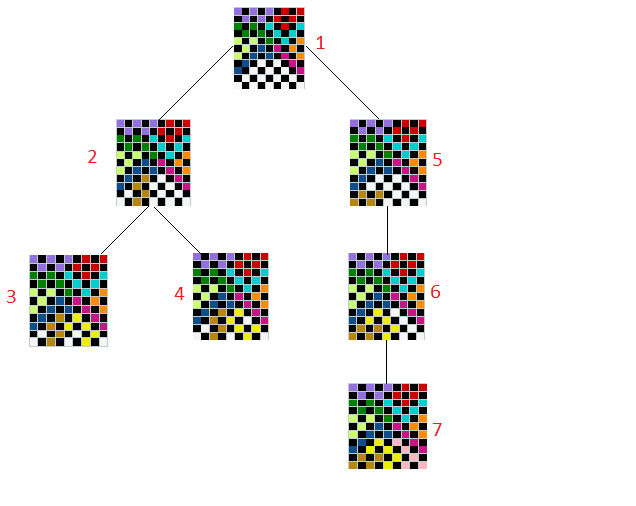
\includegraphics[scale=1]{immagini/0}
	\caption{Esempio di funzionamento dell'algoritmo DFS}
	\label{fig:0}
\end{figure}

\section{CSP}
\subsection{Descrizione}
Il secondo approccio utilizzato per risolvere questo gioco è stato formalizzare il problema in forma di CSP (Constraint Satisfaction Problem). Un CSP è composto da un insieme di variabili $X = \{X\textsubscript{1},...,X\textsubscript{n}\}$, i loro domini  $D = \{D\textsubscript{1},...,D\textsubscript{n}\}$ e un insieme di vincoli  $C = \{C\textsubscript{1},...,C\textsubscript{m}\}$, dove ogni vincolo coinvoge un sottoinsieme di variabili, specificandone una combinazione di valori permessi.\\
Uno stato è rappresentato da un assegnamento di valori ad alcune delle variabili $\{X\textsubscript{i} = v\textsubscript{i}, X\textsubscript{j} = v\textsubscript{j},...\}$.
Un assegnamento che non viola nessun vincolo è chiamato consistente, mentre un assegnamento dove ogni variabile ha un valore è detto completo. \\
La soluzione per un CSP è un assegnamento consistente e completo.

\subsection{Utilizzo}
Nella nostra implementazione il CSP è così definito:
\begin{itemize}
	\item \textbf{variabili}: tutte le forme, univocamente identificate dal loro colore;
	\item \textbf{domini}: l'insieme di valori validi per ogni variabile, dove un valore è una tupla di coordinate che identifica un possibile posizionamento di una forma nella griglia;
	\item \textbf{vincoli}: 
		\begin{itemize}
			\item nessuna variabile $X\textsubscript{i}$ deve sovrapporsi all'interno della griglia, anche solo parzialmente, con un'altra variabile $X\textsubscript{j}$;
			\item il posizionamento di una variabile nella griglia non deve creare una componente connessa con un numero di celle inferiore alla dimensione della forma più piccola, 3 nel nostro caso (vedi Figura \ref{fig:badCC}).
		\end{itemize}
\end{itemize}
\begin{figure}[h]
	\centering
	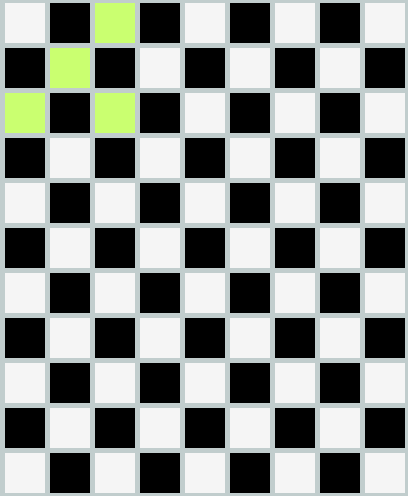
\includegraphics[scale=0.4]{immagini/badCC}
	\caption{Il quadrato in alto a sinistra forma una componente connessa di una sola cella, che è un numero inferiore alla dimensione della forma più piccola.}
	\label{fig:badCC}
\end{figure}

\subsubsection{Backtracking}
\subsubsection{Backtracking ricorsivo}
\subsubsection{MinConflict}

\subsection{Utilizzo}
\section{Nostri miglioramenti}